% ════════════════════════════════════════════
% 模型求解（5.4.4）
% ════════════════════════════════════════════
\subsubsection{结果与解读}

基于上述框架，本节依次测算付费、内容类型与内容主题的效应，并做稳健性复核。求解环境为 Python 3，读取回归阶段保存的模型系数与 HC3 协方差，参数模拟重复 1000 次，随机种子固定为 20261122。

首先给出付费效应。由表\ref{tab:q4_paid}可知，M2 的付费系数为 0.3374，HC3 标准误 0.1195，95\% 置信区间为 0.1025 至 0.5723，对应净提升 40.13\%、区间 10.80\% 至 77.24\%。在代表性画像（Photo、主题 1、7 月、周四、上午，粉丝规模 129,600 人）上，自然帖子的调整预测曝光为 40,221 次，付费帖子为 56,364 次，差值 16,142 次，区间 4,543 至 33,467 次，倍数 1.401、区间 1.104 至 1.753。全样本反事实的平均处理效应为 10,907 次，区间 3,138 至 20,195 次，倍数同样为 1.401。作为未调整的对照，原始数据中付费组的中位曝光为 12,060 次、自然组为 8,387 次，中位数比 1.438、均值比 1.405，与调整后的 1.401 非常接近，说明付费的正向差异不是由内容类型或发布时机的构成差异造成的。

\begin{longtable}{>{\centering\arraybackslash}p{0.28\textwidth}>{\centering\arraybackslash}p{0.12\textwidth}>{\centering\arraybackslash}p{0.12\textwidth}>{\centering\arraybackslash}p{0.12\textwidth}>{\centering\arraybackslash}p{0.20\textwidth}}
  \caption{付费效应测算}
  \label{tab:q4_paid} \\
  \toprule
  指标 & 估计值 & CI 下限 & CI 上限 & 说明 \\
  \midrule
  \endfirsthead
  \caption{付费效应测算（续）} \\
  \toprule
  指标 & 估计值 & CI 下限 & CI 上限 & 说明 \\
  \midrule
  \endhead
  \bottomrule
  \endfoot
  付费系数 $\beta$ & 0.3374 & 0.1025 & 0.5723 & log1p 尺度，HC3 \\
  $e^{\beta}-1$（\%） & 40.13 & 10.80 & 77.24 & 净提升百分比 \\
  自然帖子预测曝光 & 40221 & 25282 & 62189 & 代表性画像，烟雾还原 \\
  付费帖子预测曝光 & 56364 & 36172 & 87327 & 同一画像，$X_7=1$ \\
  差值（次） & 16142 & 4543 & 33467 & 付费减自然 \\
  倍数 & 1.401 & 1.104 & 1.753 & 付费除以自然 \\
  全样本 ATE 差值（次） & 10907 & 3138 & 20195 & 500 条逐条反事实 \\
  全样本 ATE 倍数 & 1.401 & 1.104 & 1.753 & 反事实均值之比 \\
  原始付费组中位曝光 & 12060 & — & — & $n=139$，未调整 \\
  原始自然组中位曝光 & 8387 & — & — & $n=361$，未调整 \\
  原始中位数比 & 1.438 & — & — & 未调整对照 \\
  原始均值比 & 1.405 & — & — & 未调整对照 \\
\end{longtable}

在解读付费系数前，图\ref{fig:q4_balance}核对两组可比性。左上图把两组粉丝规模对数的提琴图、箱线与散点并排，自然组与付费组的均值分别为 11.711 与 11.715，标准化均值差仅 0.031，两个分布几乎完全重叠；右上图逐月给出付费占比与 Wilson 95\% 区间，各月在 16.0\% 至 40.0\% 之间波动，整体线 27.8\% 落在多数月份的区间内；左下与右下分别给出类型与主题构成，Photo 在两组都占 85\% 以上，主题构成的差异不超过 4.2 个百分点。唯一可见的差异是付费组 Video 占 2.9\%、自然组仅 0.8\%，但 Video 总共只有 7 条，且回归已用类型哑变量吸收其影响。由此可见，两组在可观测特征上接近，后文 40.13\% 的提升不太可能由粉丝规模或内容构成差异解释。

\begin{figure}[ht]
  \centering
  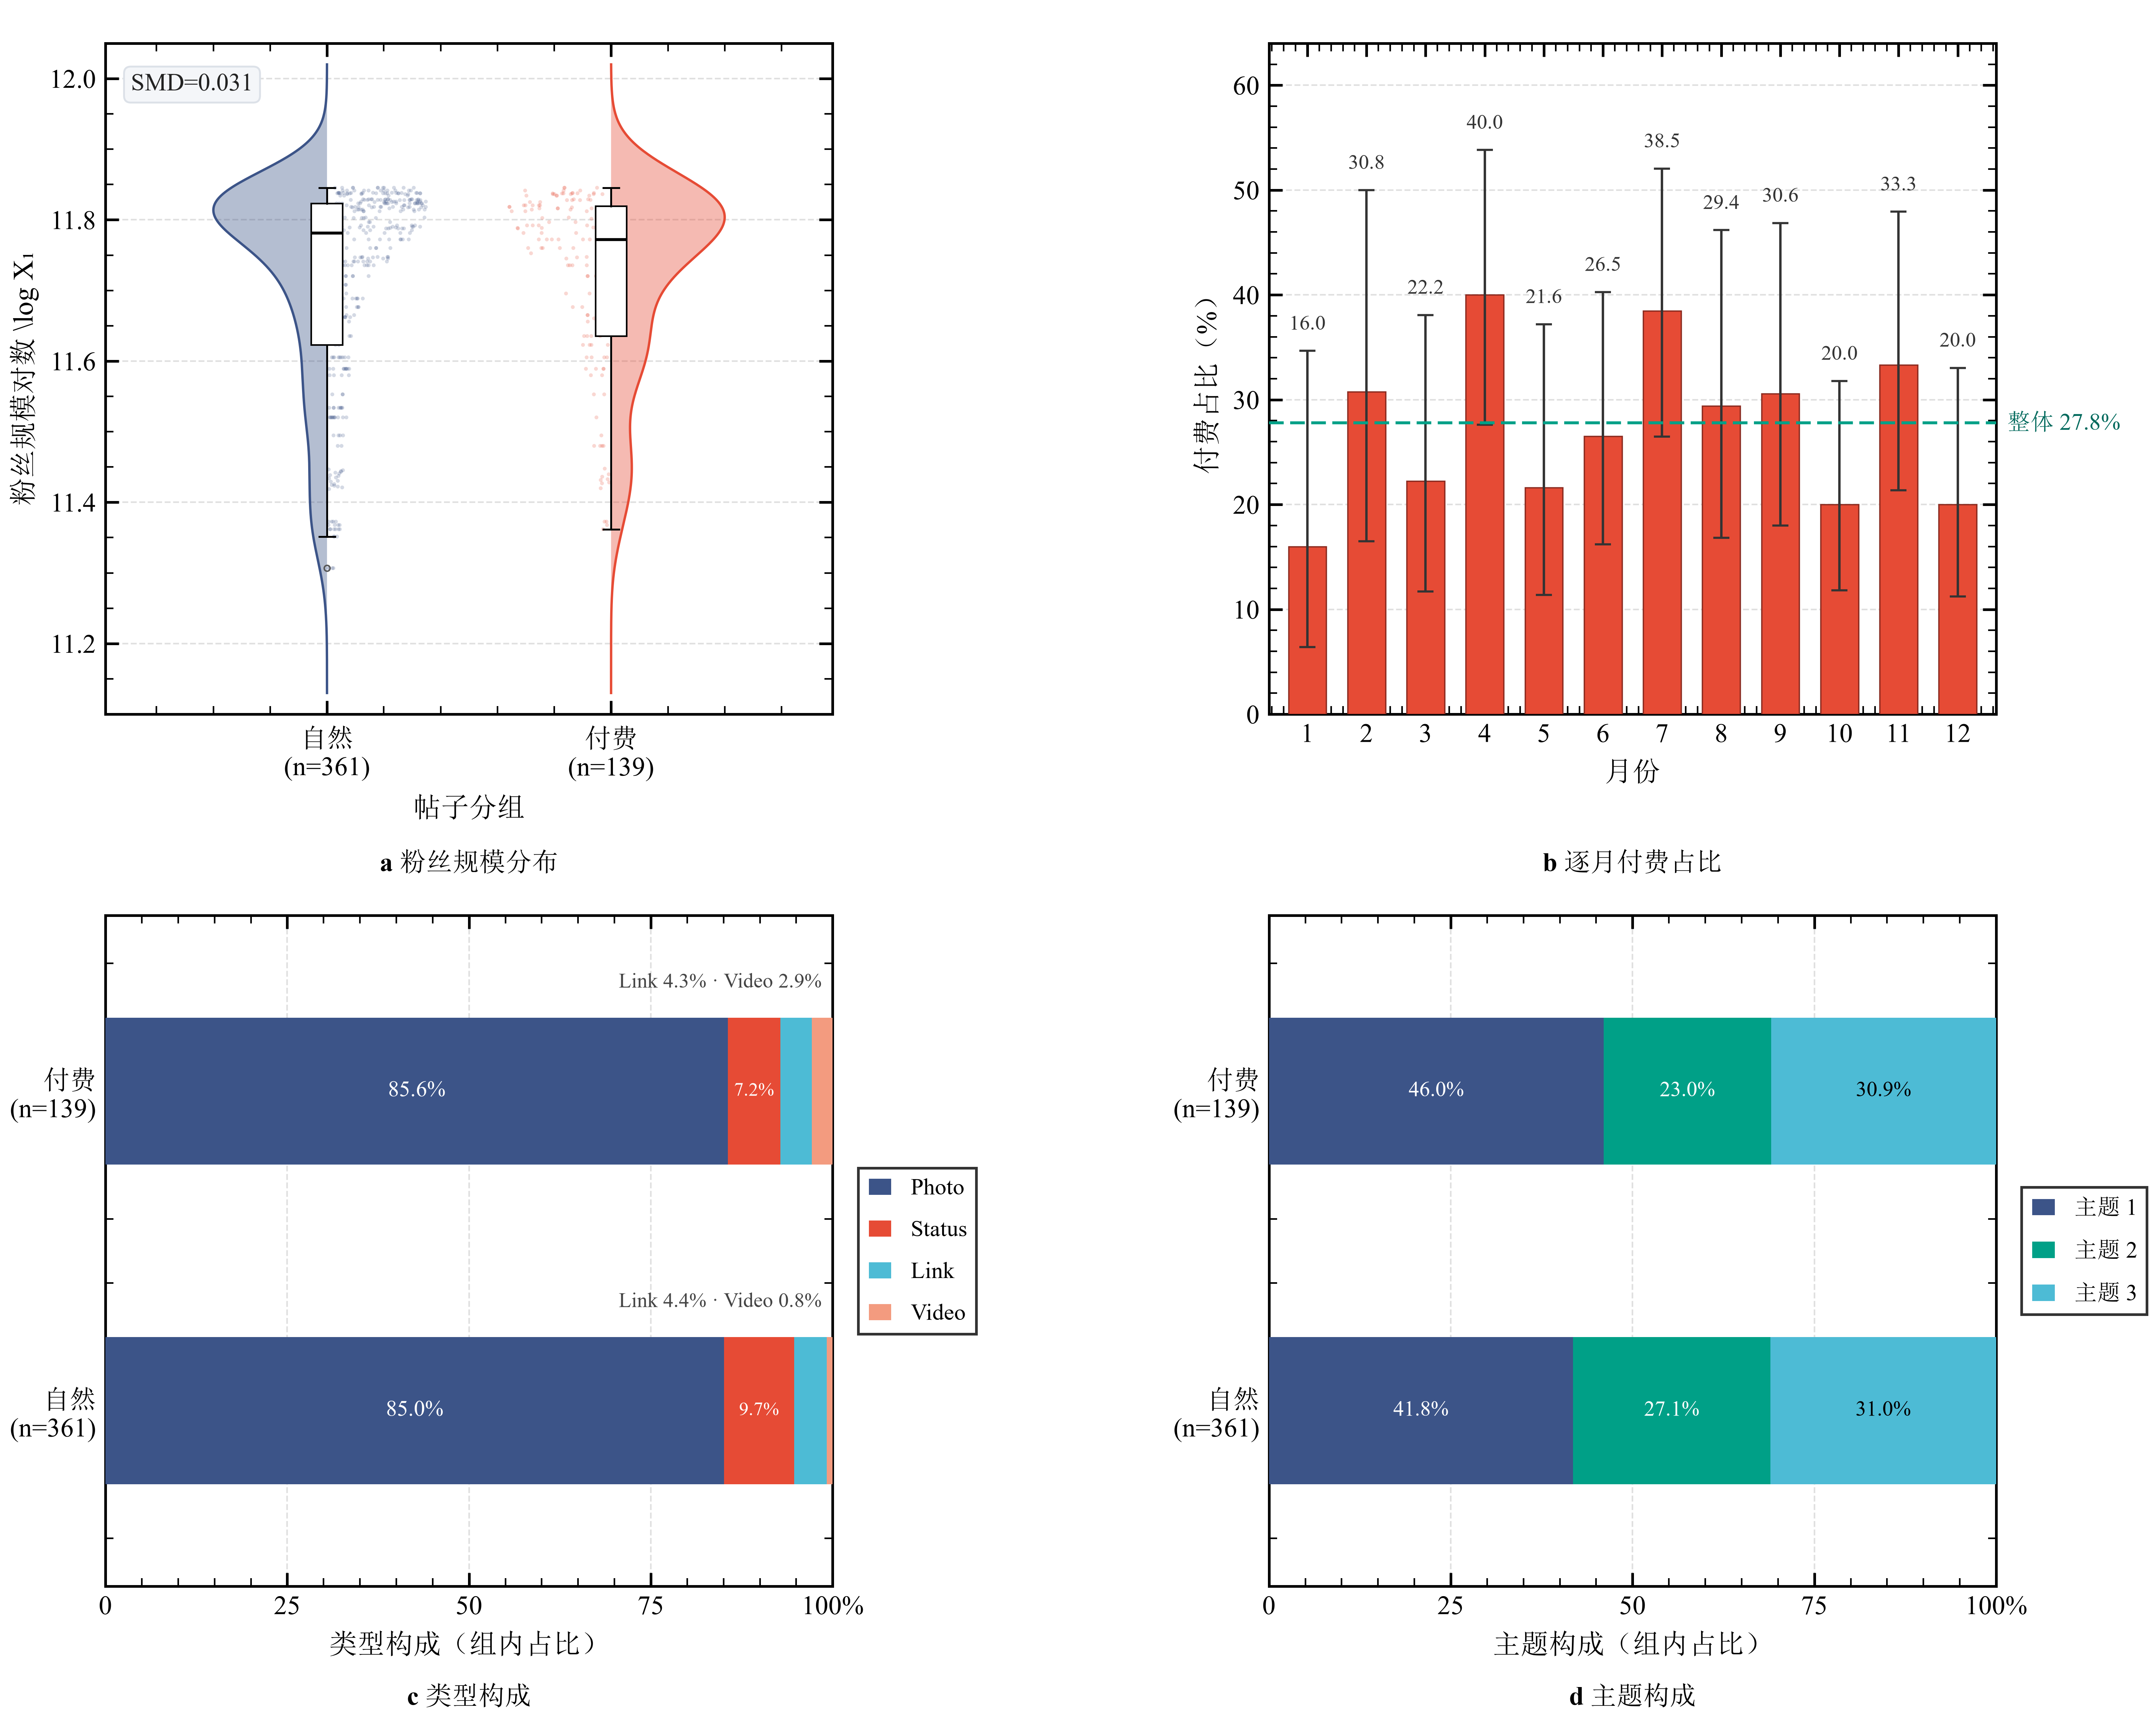
\includegraphics[width=0.80\textwidth]{../求解/临时产物/补充图3_付费可比性.png}
  \caption{付费组与自然组的可比性}
  \label{fig:q4_balance}
\end{figure}

其次比较四种内容类型。表\ref{tab:q4_type}以 Photo 为参照，Video 的系数为 1.5896、p 值 0.0001，折算为 4.90 倍，区间 2.23 至 10.79；Status 的系数为 1.1538、p 值小于 0.001，折算为 3.17 倍，区间 2.49 至 4.04；Link 的系数为 0.1215、p 值 0.643，折算为 1.13 倍，区间 0.68 至 1.89，与 Photo 无显著差异。在自然帖、主题 1、7 月、周四、上午、粉丝规模 129,600 人的代表性画像上，Video 的调整预测曝光为 197,157 次，比 Photo 的 40,221 次多出约 15.7 万次；Status 为 127,511 次，Link 为 45,420 次。Video 的倍数最高，但其区间上限约为下限的 4.8 倍，且样本只有 7 条，解读时应把它理解为“方向明确、幅度不确定”的信号，而不是精确的投放回报。

\begin{longtable}{>{\centering\arraybackslash}p{0.15\textwidth}>{\centering\arraybackslash}p{0.08\textwidth}>{\centering\arraybackslash}p{0.08\textwidth}>{\centering\arraybackslash}p{0.075\textwidth}>{\centering\arraybackslash}p{0.075\textwidth}>{\centering\arraybackslash}p{0.09\textwidth}>{\centering\arraybackslash}p{0.09\textwidth}>{\centering\arraybackslash}p{0.08\textwidth}}
  \caption{内容类型效应}
  \label{tab:q4_type} \\
  \toprule
  对比 & 系数 & HC3\newline 标准误 & p 值 & 倍数 & 倍数下限 & 倍数上限 & 处理组\newline 曝光 \\
  \midrule
  \endfirsthead
  \caption{内容类型效应（续）} \\
  \toprule
  对比 & 系数 & HC3\newline 标准误 & p 值 & 倍数 & 倍数下限 & 倍数上限 & 处理组\newline 曝光 \\
  \midrule
  \endhead
  \bottomrule
  \endfoot
  Video 对 Photo & 1.5896 & 0.4017 & 0.0001 & 4.902 & 2.226 & 10.793 & 197157 \\
  Status 对 Photo & 1.1538 & 0.1235 & $<$0.001 & 3.170 & 2.487 & 4.041 & 127511 \\
  Link 对 Photo & 0.1215 & 0.2619 & 0.643 & 1.129 & 0.675 & 1.889 & 45420 \\
\end{longtable}

图\ref{fig:q4_pred}把上述调整预测与内容主题的结果放在同一张图中。左上图显示付费与自然的区间在曝光尺度上有重叠，但点估计的差值明确为正；右上图按类型排列，Video 的点估计远高于其他三类，区间也最宽；左下图显示主题 2 的调整预测最低，主题 1 最高；右下图按付费与类型分组给出观测中位数，四条连线都向上倾斜，但斜率差异不大，交互检验的 p 值为 0.531，说明付费效应在不同内容类型之间没有显著差异，主效应模型已经足够。

\begin{figure}[ht]
  \centering
  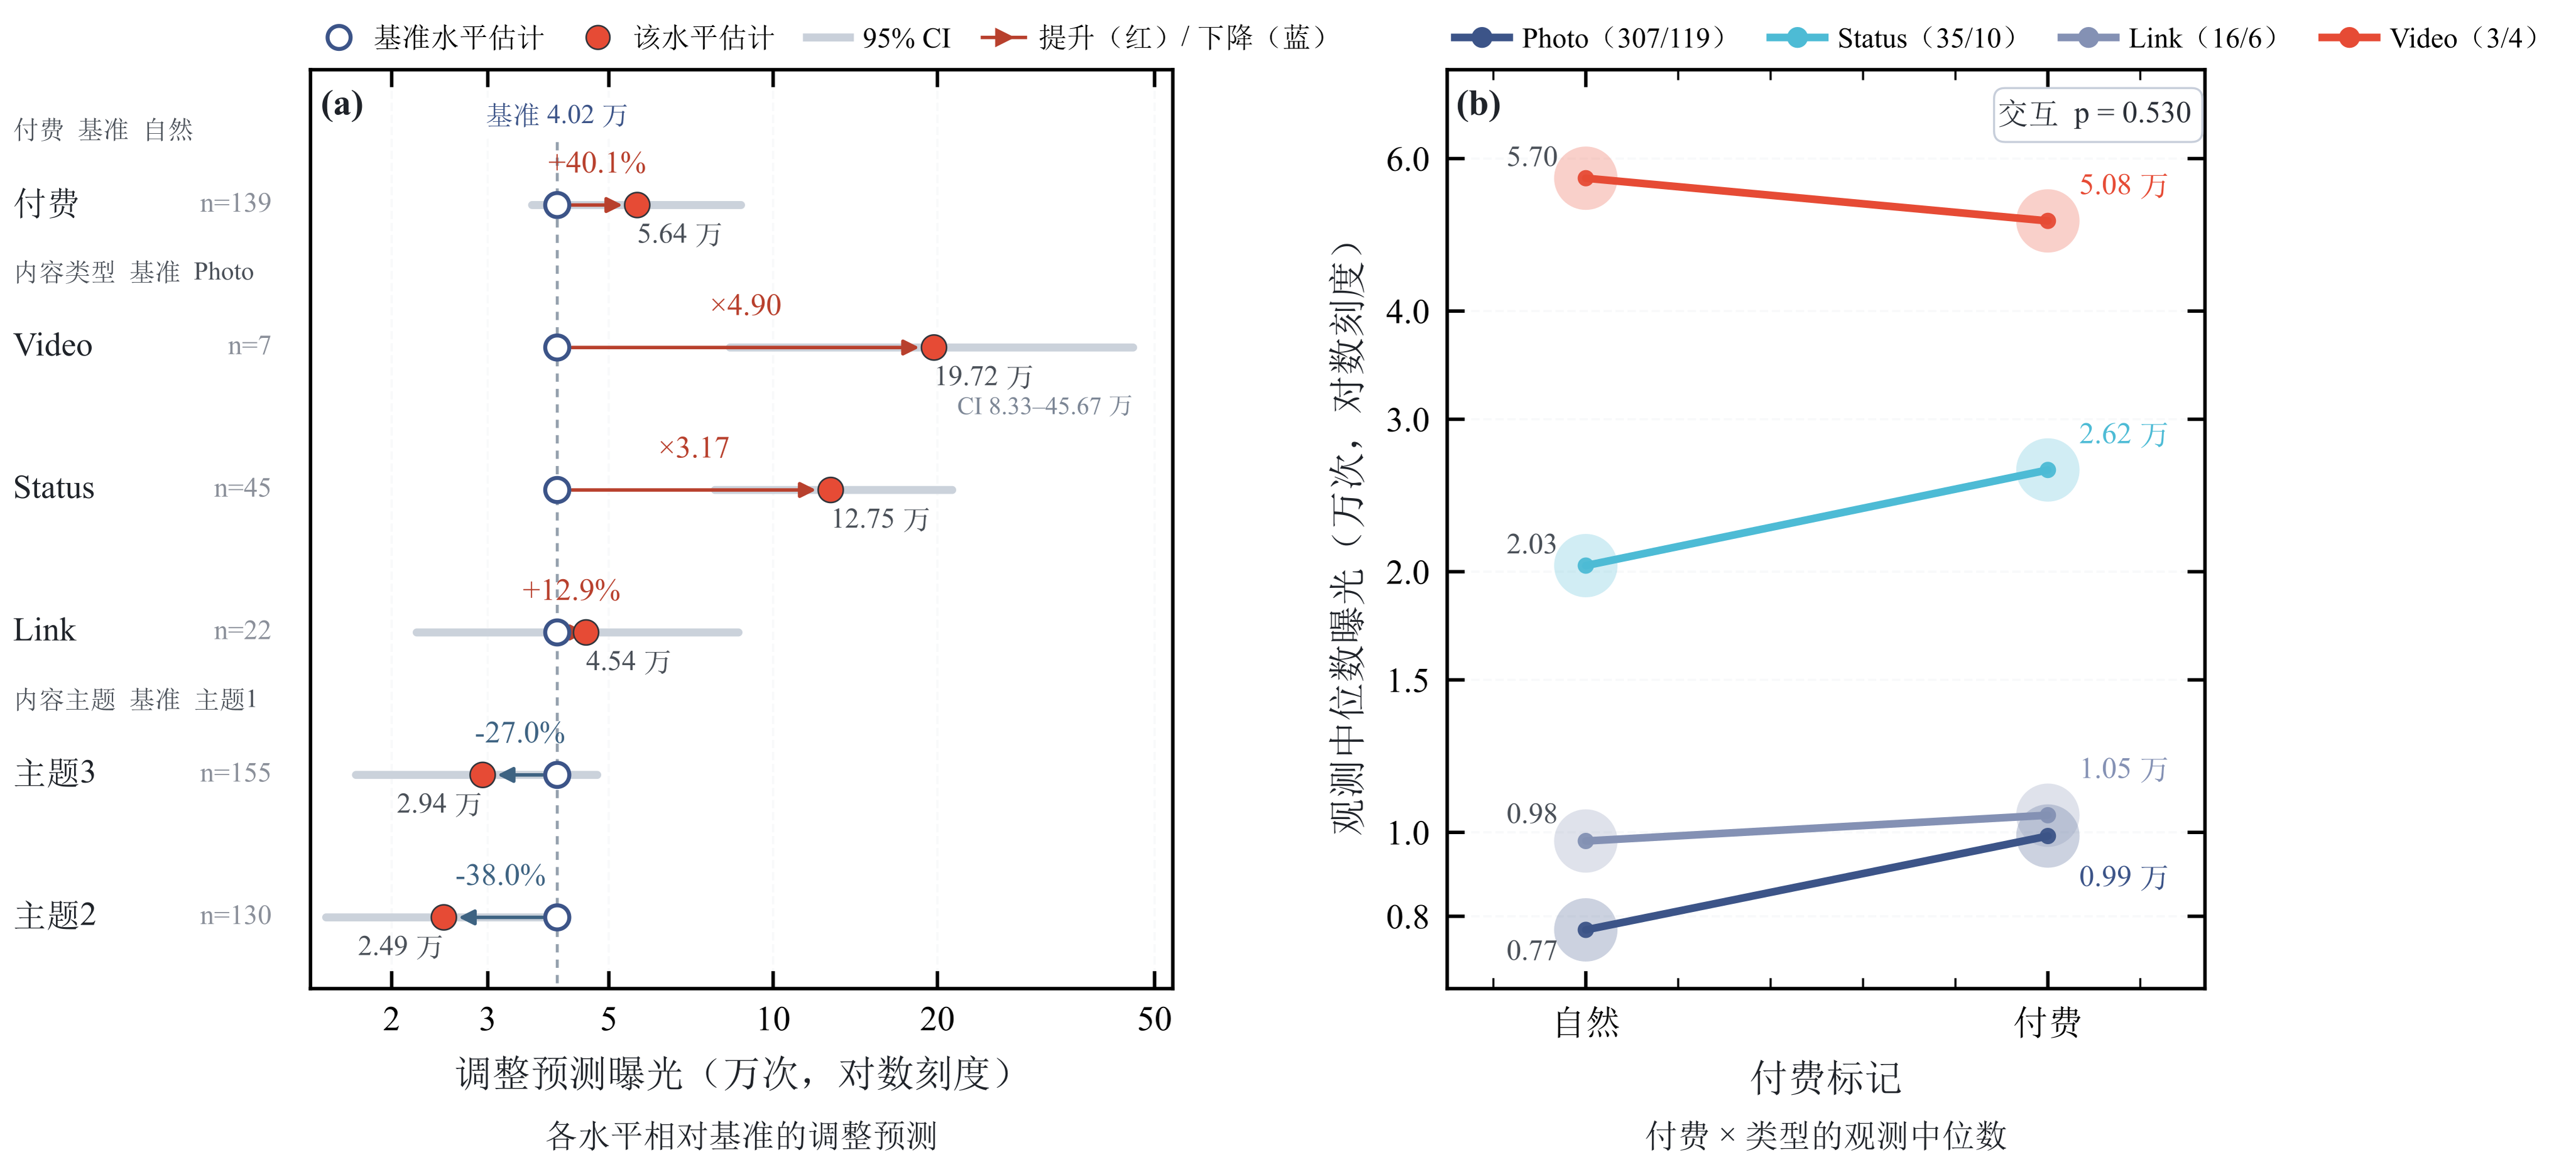
\includegraphics[width=0.70\textwidth]{../求解/问题四/结果/图11_调整预测效应.png}
  \caption{付费、内容类型与内容主题的调整预测曝光}
  \label{fig:q4_pred}
\end{figure}

再次检验内容主题。表\ref{tab:q4_theme}报告联合与两两结果。联合 Wald 统计量为 12.6783、自由度 2、p 值 0.0018，拒绝“两个主题哑变量同时为零”的原假设，说明主题整体对曝光有显著影响。相对主题 1，主题 2 的系数为 $-0.4784$、折算 0.620 倍，区间 0.475 至 0.808；主题 3 的系数为 $-0.3147$、折算 0.730 倍，区间 0.561 至 0.950。两者都显著低于主题 1，且主题 2 的点估计更低。但主题 2 与主题 3 的直接差异为 $-0.1638$、p 值 0.186、倍数 0.849，区间 0.666 至 1.082，在 5\% 水平不显著，不能据此断言主题 2 一定劣于主题 3。

\begin{longtable}{>{\centering\arraybackslash}p{0.20\textwidth}>{\centering\arraybackslash}p{0.10\textwidth}>{\centering\arraybackslash}p{0.10\textwidth}>{\centering\arraybackslash}p{0.09\textwidth}>{\centering\arraybackslash}p{0.09\textwidth}>{\centering\arraybackslash}p{0.09\textwidth}>{\centering\arraybackslash}p{0.09\textwidth}}
  \caption{内容主题效应与两两对比}
  \label{tab:q4_theme} \\
  \toprule
  对比 & 系数或\newline 统计量 & 标准误 & p 值 & 倍数 & 倍数下限 & 倍数上限 \\
  \midrule
  \endfirsthead
  \caption{内容主题效应与两两对比（续）} \\
  \toprule
  对比 & 系数或\newline 统计量 & 标准误 & p 值 & 倍数 & 倍数下限 & 倍数上限 \\
  \midrule
  \endhead
  \bottomrule
  \endfoot
  主题联合 Wald & 12.6783 & — & 0.0018 & — & — & — \\
  主题 2 对主题 1 & $-0.4784$ & 0.1352 & 0.0004 & 0.620 & 0.475 & 0.808 \\
  主题 3 对主题 1 & $-0.3147$ & 0.1337 & 0.0190 & 0.730 & 0.561 & 0.950 \\
  主题 2 对主题 3 & $-0.1638$ & 0.1239 & 0.1864 & 0.849 & 0.666 & 1.082 \\
\end{longtable}

最后做稳健性复核。表\ref{tab:q4_robust}汇总六种设定下的付费与视频效应。付费提升在 M1 至 M4 中为 40.09\% 至 49.65\%，Huber 回归为 37.44\%，Gamma 模型为 44.84\%，全部在 1\% 水平显著；Video 倍数在 3.52 至 5.41 之间，同样全部显著。M3 与 M4 因未使用月份固定效应，付费系数略高，说明月份控制吸收了一部分与付费相关的季节差异；Gamma 模型的 Video 倍数最低，反映其对右偏分布的拟合更保守。六种设定的方向一致、区间都不跨过 0 或 1，可以认为结论不依赖单一模型设定。

\begin{longtable}{>{\centering\arraybackslash}p{0.24\textwidth}>{\centering\arraybackslash}p{0.10\textwidth}>{\centering\arraybackslash}p{0.09\textwidth}>{\centering\arraybackslash}p{0.11\textwidth}>{\centering\arraybackslash}p{0.09\textwidth}>{\centering\arraybackslash}p{0.08\textwidth}>{\centering\arraybackslash}p{0.09\textwidth}}
  \caption{效应稳健性对比}
  \label{tab:q4_robust} \\
  \toprule
  设定 & 付费系数 & 付费 p 值 & 付费提升\newline （\%） & Video\newline 系数 & Video\newline p 值 & Video\newline 倍数 \\
  \midrule
  \endfirsthead
  \caption{效应稳健性对比（续）} \\
  \toprule
  设定 & 付费系数 & 付费 p 值 & 付费提升\newline （\%） & Video\newline 系数 & Video\newline p 值 & Video\newline 倍数 \\
  \midrule
  \endhead
  \bottomrule
  \endfoot
  M1 全模型 & 0.3371 & 0.005 & 40.09 & 1.5881 & $<$0.001 & 4.894 \\
  M2 月份固定效应 & 0.3374 & 0.005 & 40.13 & 1.5896 & $<$0.001 & 4.902 \\
  M3 仅 $\log X_1$ & 0.4031 & 0.001 & 49.65 & 1.6583 & $<$0.001 & 5.250 \\
  M4 $\log X_1$ 加线性月份 & 0.3862 & 0.002 & 47.14 & 1.6878 & $<$0.001 & 5.408 \\
  Huber 稳健回归 & 0.3180 & 0.001 & 37.44 & 1.6834 & $<$0.001 & 5.384 \\
  Gamma 广义线性模型 & 0.3705 & 0.010 & 44.84 & 1.2579 & 0.001 & 3.518 \\
\end{longtable}

图\ref{fig:q4_robust}以森林图形式展示稳健性。左图横轴为付费带来的百分比提升，六行点估计集中在 37\% 至 50\% 之间，红色标注的最终模型 M2 位于中间，虚线 0 位于所有区间之外；右图横轴为 Video 相对 Photo 的倍数，采用对数刻度，虚线 1 表示无差异，六行点估计集中在 3.5 至 5.4 之间，最终模型接近中位。两张图都没有出现方向反转或区间跨过参考线的情况，说明付费与视频的正向效应在不同设定下稳定存在。

\begin{figure}[ht]
  \centering
  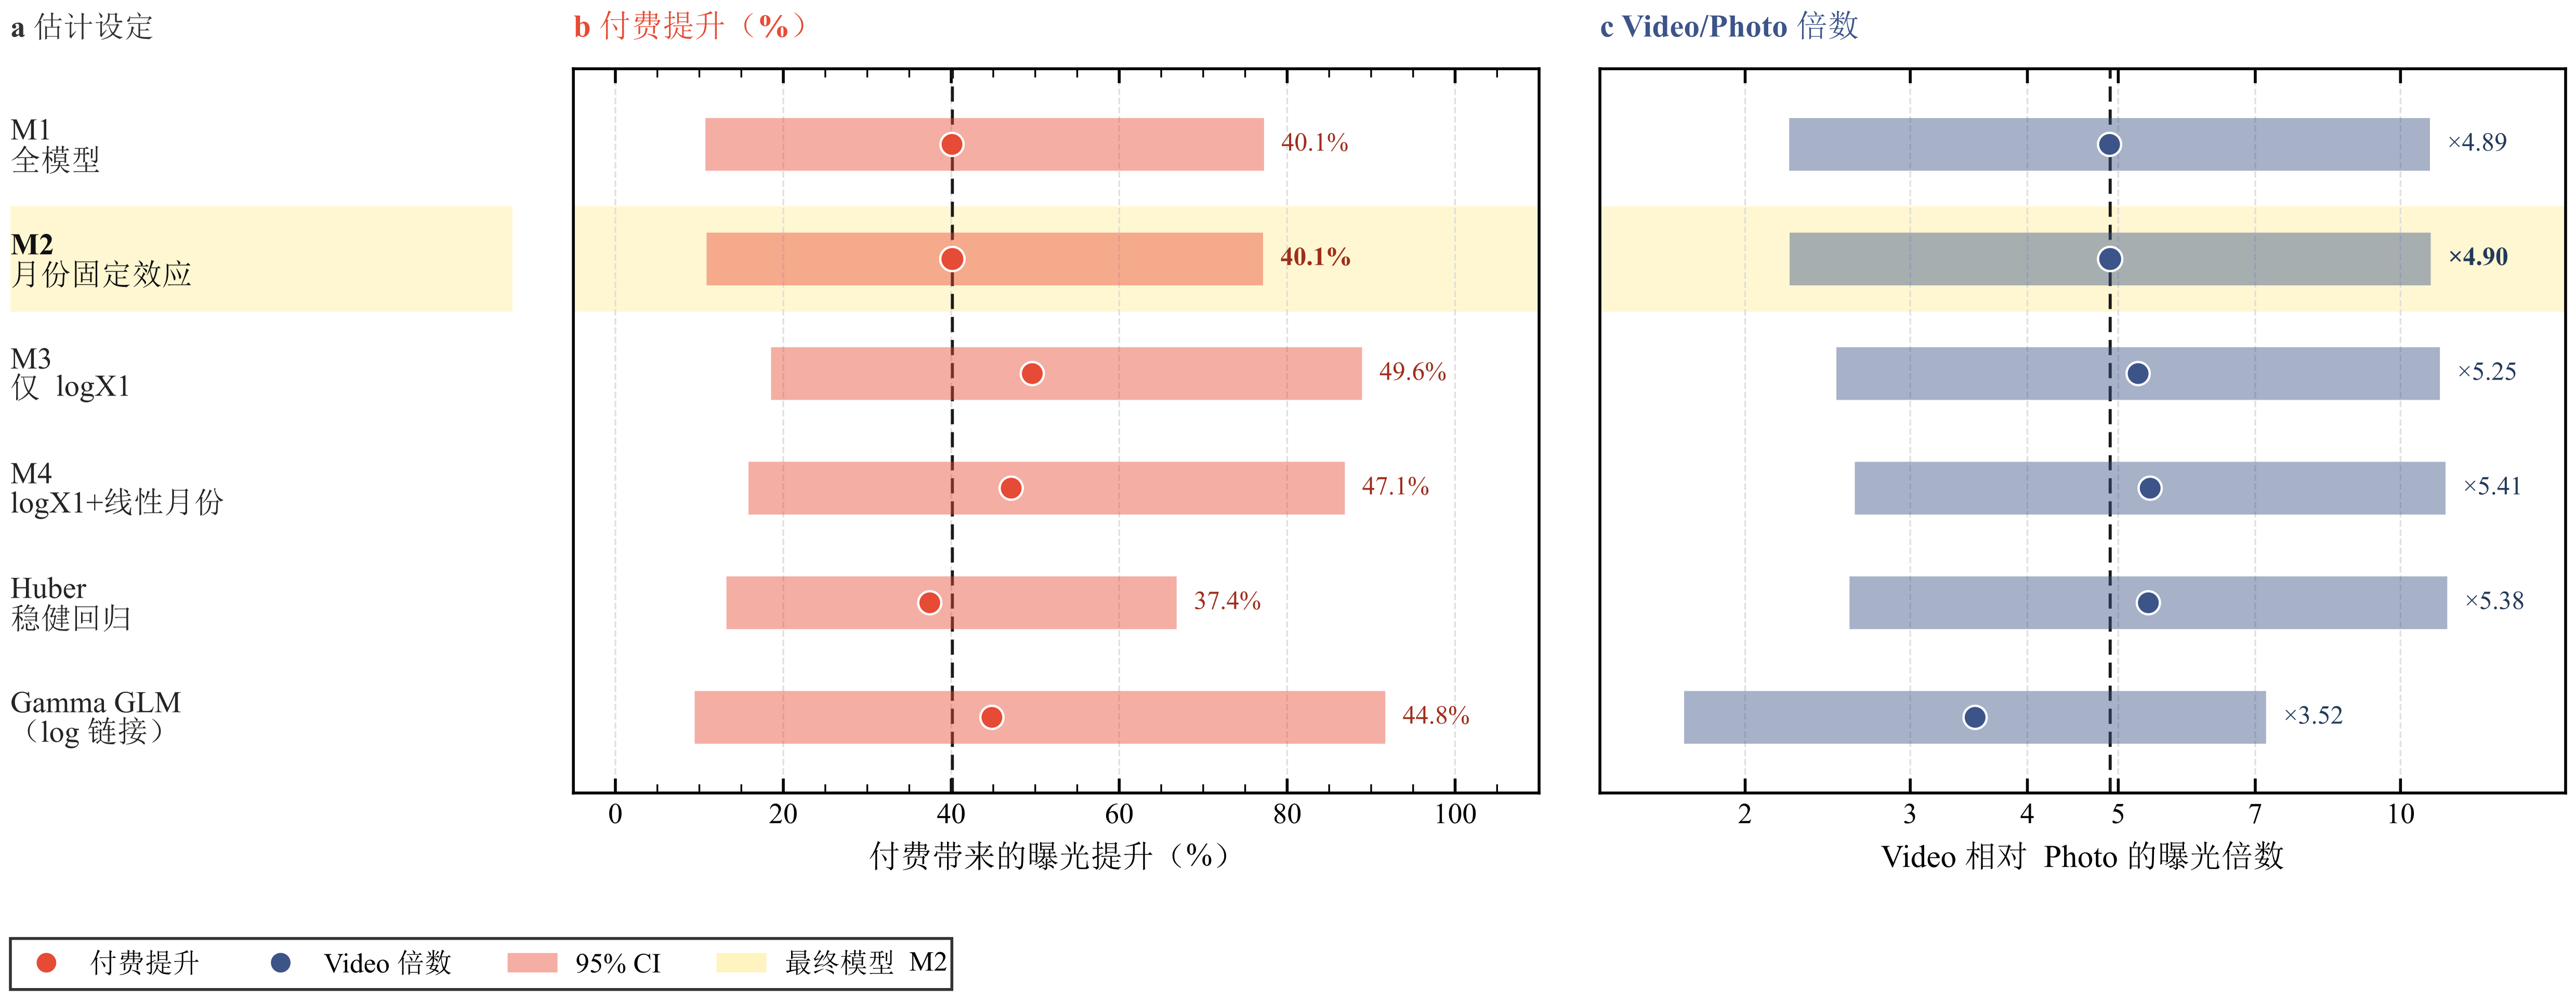
\includegraphics[width=0.75\textwidth]{../求解/问题四/结果/图12_效应稳健性.png}
  \caption{付费与视频效应在六种设定下的稳健性}
  \label{fig:q4_robust}
\end{figure}

综合以上结果，付费带来约 40\% 的曝光提升，代表性画像上约为 1.6 万次增量；视频相对图片约为 4.9 倍，方向明确但精度受 7 条样本限制；状态类型约为 3.2 倍，链接类型与图片无显著差异；内容主题整体显著，主题 2 与主题 3 都低于主题 1，但两者之间差异不显著。上述结论在六种模型设定下保持一致，可作为品牌主页内容编排与付费投放的参考。
